\chapter{The output mode cleaner}
\label{ch:omc}
One of the primary components of the Enhanced LIGO upgrade was the addition of an output mode cleaner or OMC \cite{T060156}. %NL%
This chapter describes the motivation for installing and OMC and some measurements of the performance of the OMC installed on the H1 interferometer at the LIGO Hanford Observatory.

\section{Motivation for an OMC}
The interferometer is supplied with a beam that has a very nearly pure Gaussian spatial profile thanks to the input mode cleaner. %NL%
The input mode cleaner is a nearly critically coupled resonant optical cavity which filters the beam supplied by the laser before it is delivered to the interferometer input. %NL%
The power recycling cavity builds up power and delivers it to the long arms. %NL%
The arms further recycle the laser light and this large resonant field acts as the source field that gets modulated by a passing gravitational wave and pumps light into sidebands at the gravitational wave frequency. %NL%
The gravitational wave signal on the PD comprises the beat note of these audio frequency sidebands with a strong coherent field. %NL%
Although the beam delivered by the input mode cleaner is spatially very pure, the efficiency of coupling this beam to the final resonant mode of the arm cavity is not ideal. %NL%
Components of the input light that are not matched to the mode of the arm cavity will not resonate and some of this unmatched light will exit the antisymmetric port along with the signal light. %NL%
The unmatched light at the antisymmetric port will exist as higher order modes (HOM) relative to the arm cavity mode and is often referred to as ``junk light.'' %NL%
The presence of this light on a photodetector will contribute photon shot noise. %NL%
Also, if the coupling is time dependent, the time variation of the junk light directly contaminate the signal with noise.

It is, therefore, desirable to be able to separate the junk light from the signal rich audio frequency fields originating in the arm cavities. %NL%
A critically coupled resonant optical cavity is a natural spatial filter for light. %NL%
When placed at the output of the interferometer between the AS port and the PD, as seen in Figure \ref{fig:omclocation}, we refer to such a cavity as the output mode cleaner (OMC).

\begin{figure}
  \begin{center}
  \leavevmode
  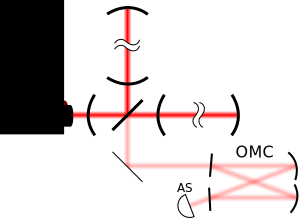
\includegraphics{figs-omc/omclocation.pdf}
  \end{center}
  \caption[Diagram showing the location of the OMC.]{Diagram showing the location of the OMC. This diagram is not drawn to scale.}
  \label{fig:omclocation}
\end{figure}

It can be useful to point out that interferometers based on both RF and DC readout can benefit from an OMC. %NL%
Both the GEO and Virgo interferometers have used OMCs in an RF readout configuration, and LIGO experimented with an OMC before using DC readout \cite{G040326}. %NL%
An OMC is especially important for a DC readout interferometer because any audio frequency modulation of fields that are not the local oscillator or signal will contaminate the readout. %NL%
Because readout is performed at DC, all audio frequency interference of the fields will directly couple to the signal channel, as opposed to an RF heterodyne scheme where the signal is shifted away from low frequency interference. %NL%
An OMC may also be used to ensure that the light provided by the differential arm offset dominates the DC power present on the detection photodiode, otherwise DC power from other fields (such as the RF sidebands) will contribute to photon shot noise without increasing the signal strength. %NL%


Thus, for an interferometer that employs DC readout, the OMC should efficiently strip the HOM field components of the carrier field as well as the RF sidebands. %NL%
This is achieved by creating a cavity with a narrow linewidth, capable of transmitting the desired (carrier) field, while filtering out higher frequencies. %NL%
Ideally, being a critically coupled optical cavity, light incident on the OMC is totally transmitted on resonance. %NL%
The normalized transmission of the off-resonant fields is given by
\begin{equation}
\label{eqn:finesse}
\frac{T}{T_0}=\frac{1}{1+\frac{4}{\pi^2}\mathcal{F}^2\sin{}^2\phi},
\end{equation}
where $\mathcal{F}$ is known as the \emph{cavity finesse} (see also Section \ref{sec:finesse}) and $\phi$ is the detuning from resonance. %NL%
In terms of a frequency detuning of $\Delta f$ of the incident light, $\phi = \pi \Delta f / \mathrm{FSR}$. %NL%
The FSR is the frequency spacing of successive resonances, discussed in Section \ref{sec:FSR}.

\section{Optical and mechanical design of the OMC}
\begin{figure}
  \begin{center}
  \leavevmode
  \includegraphics{figs-omc/omcphoto.pdf}
  \end{center}
  \caption[Photograph of the OMC.]{Photograph of the OMC. The strong red line shows the primary beam path. The light red line shows the QPD sample of the input beam. Only shown are the QPD and transmission PD tombstones, the actual photodetectors are not mounted in this photograph. Photograph credit to Sam Waldman.}
  \label{fig:omcphoto}
\end{figure}
Prior to Enhanced LIGO, experiments were performed using a OMC borrowed from the GEO600 interferometer to investigate the difficulties in using an OMC with LIGO. %NL%
Noise introduced from jitter of the OMC input beam due to air currents and mechanical vibrations spoiled the sensitivity of the LIGO detector when the OMC was used. %NL%
Consequently, one of the most obvious lessons learned from these investigations was the need to house the OMC in a low vibration environment. %NL%
For Enhanced LIGO, it was decided that the OMC would be housed inside the vacuum system and would be isolated from vibrations of the environment through the use of a seismically isolated optics table as well as a suspension system to provide passive filtering of vibrations.

\subsection{Cavity optics}
The design of the OMC was chosen to be a four mirror bow-tie cavity. %NL%
This choice was made over that of a two mirror linear cavity so that there was spatial separation of the reflected beam. %NL%
An even number of mirrors was chosen such that the horizontal and vertical HOMs would experience the same overall phase shift and thus experience nearly the same frequency offset from resonance, reducing the chances of an accidental HOM resonance.

\begin{figure}
  \begin{center}
  \leavevmode
  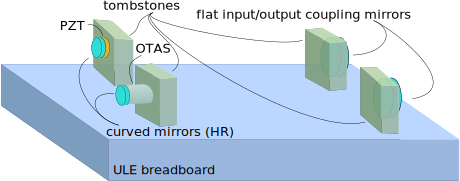
\includegraphics{figs-omc/construction.pdf}
  \end{center}
  \caption[Diagram of OMC cavity components]{Diagram of OMC cavity components. Auxiliary optics and sensors are not shown. The tombstones have holes (not pictured) machined in them to allow the laser beam to pass through (see Figure \ref{fig:inputcouplerphoto} for a photograph of the input coupler and tombstone.)}
  \label{fig:omcconstruction}
\end{figure}

\begin{figure}
  \begin{center}
  \leavevmode
  \includegraphics{figs-omc/inputcouplerphoto.pdf}
  \end{center}
  \caption[Close up photograph of the OMC input coupler mirror.]{Close up photograph of the OMC input coupler mirror. The photograph is taken from the in-cavity side of the optic.}
  \label{fig:inputcouplerphoto}
\end{figure}

A diagram of the OMC may be seen in Figure \ref{fig:omcconstruction}. %NL%
The OMC optics are bonded with Vacseal epoxy onto custom designed fused silica optics mounts, called tombstones. %NL%
 The tombstones were then bonded to a slab of Corning ultra-low expansion (ULE) Glass\footnote{The dimensions of the OMC breadboard are 450mm$\times$150mm$\times$39mm} with UV cure epoxy from Optocast, which we will refer to as the \emph{OMC breadboard}, pictured in Figure \ref{fig:omcphoto}. %NL%
Figure \ref{fig:inputcouplerphoto} shows the OMC input coupler mirror and tombstone, bonded to the breadboard. %NL%
This arrangement fixed the cavity length to the desired value and was designed to be stable against thermal variation. %NL%
The microscopic cavity length was controlled using a pair of actuators. %NL%
A fast PZT between one of the optics and its tombstone acted as a low range (1/10 of a wavelength) high bandwidth (5kHz) length actuator. %NL%
Long range (several wavelengths) actuation was provided by one cavity mirror situated at the end of an aluminum tube heated by a ceramic heating element, affectionately referred to as the OTAS.\footnote{OMC Thermal Actuation System}

A mode cleaner cavity is purposefully designed such that HOMs do not occupy a degenerate resonance with the resonant \TEM{00} mode (see Section \ref{sec:modecleanap} on how a mode cleaner acts as a filter of transverse modes). %NL%
Cavities are commonly characterized by their stability $g$-parameter.\footnote{Asymmetric cavities are often given two $g$-parameters, one for each mirror (labeled 1 and 2) and $g=\sqrt{g_1 g_2}$.} The Gouy phase shift, $\eta$, is the phase shift of a focused \TEM{00} beam relative to a plane electromagnetic wave. %NL%
The round trip Gouy shift in the cavity is determined by the cavity geometry as
\begin{equation}
\label{eqn:gouyg}
\cos(\eta)=g,
\end{equation}
where the $g$-parameter is usually given by $g=1-L/R$ for a linear cavity of length $L$ and mirror radius of curvature $R$ \cite{T080208}. %NL%
The OMC is not a linear cavity, the light travels the length of the cavity only once during a full round trip. %NL%
To avoid confusion we will use the \emph{perimeter}, $p$, to denote the full round trip length. %NL%
One may substitute $2L=p$ in most formulae for linear cavities. %NL%
An extensive analysis was done by Sam Waldman to determine the optimal cavity geometry to minimize the transmission of off-resonant HOM and frequency components through the OMC \cite{T080144}. %NL%
The final design of the OMC was chosen to have a perimeter length of 1.042m, with 2m radius of curvature curved optics, giving a $g$-parameter of 0.7395 and a Gouy phase shift of $0.235\pi$ radians. %NL%
This implies that the fourth-order HOMs will accumulate almost $\pi$ radians relative to the \TEM{00} mode and be somewhat close to resonance.

\subsection{Sensors and auxiliary optics}

The gravitational wave signal readout is derived from the OMC transmitted power. %NL%
The light transmitted by the OMC is split by a near 50/50 beam splitter and detected on two photodiodes. %NL%
Both the beam splitter and photodiodes are located on the OMC breadboard. %NL%
The beamsplitter is glued to a tombstone similar to that of the cavity optics. %NL%
The photodiodes were attached to tombstones via a sandwich of metal plates screwed together around the tombstone. %NL%
This arrangement ensured that the OMC transmitted beam would not drift relative to the readout detectors.

A steering mirror on the OMC breadboard transmitted a small sample of the incoming beam allowing the input pointing to be analyzed by two quadrant photodetectors (QPDs). %NL%
A 50/50 beam splitter distributed equal amounts of the input beam to the two QPDs. %NL%
The QPDs were located at different distances from the beam splitter to allow both beam angle and lateral position to be measured. %NL%
The location of all the OMC sensors can be seen in Figure \ref{fig:omcphoto}.

\subsection{Suspension system}
\begin{figure}
  \begin{center}
  \leavevmode
  \includegraphics{figs-omc/susphoto.pdf}
  \end{center}
  \caption[Photograph of the OMC double pendulum suspension.]{Photograph of the OMC double pendulum suspension. The line sketch shows the upper mass stage, which is obscured in the photograph by the coil actuators.}
  \label{fig:susphoto}
\end{figure}

The OMC breadboard was suspended from a two stage vibration isolation suspension, pictured in Figure \ref{fig:susphoto}. %NL%
On the optics table was a large steel frame which housed the OMC. %NL%
An upper mass stage was suspended from the frame by two pendulum wires attached to the ends of blade springs. %NL%
The OMC breadboard was then suspended by four more wires attached to blade springs from the upper mass stage. %NL%
Servo control provided feedback damping of the suspension eigenmodes. %NL%
All actuation and sensing was performed on the intermediate stage, with actuation provided by electromagnetic coil actuators attached to the cage which applied forces to permanent magnets attached to the upper mass. %NL%
The actuator module also housed the sensing system which consisted of LED shadow sensors which measured the position of protruding flags attached to the magnets used for actuation.

\subsection{Mode matching telescope}
\begin{figure}
  \begin{center}
  \leavevmode
  \includegraphics{figs-omc/ttphoto.pdf}
  \end{center}
  \caption[Photograph of a Tip Tilt optic.]{Photograph of a Tip Tilt optic. The original Tip Tilt design is shown, before being retrofitted with blade springs. Alignment actuation control is provided by coil actuators coupled to permanent magnets housed in the mirror holder. }
  \label{fig:ttphoto}
\end{figure}
The beam exiting the interferometer from the antisymmetric port was directed through a beam steering and mode matching telescope. %NL%
The purpose of such a telescope is to correctly align and focus the beam exiting the interferometer to maximize the transmission of the gravitational wave signal through the OMC.

The steering optics were housed in a single pendulum suspension system. %NL%
The suspension and optics were collectively referred to as \emph{Tip-Tilt optics},\footnote{The Tip Tilts were designed by B. %NL%
Slagmolen of the Australian National University\cite{T0900096}.} one of which is pictured in Figure \ref{fig:ttphoto}. %NL%
The mounting and suspension of the beam steering optics underwent several modifications during the Enhanced LIGO project (see Chapter \ref{ch:jitter}). %NL%
The final configuration consisted of three highly reflective curved mirrors. %NL%
Two suspended by a single pendulum stage, with vertical isolation provided by blade springs, and a coil-magnet/shadow sensor system similar to that used in the OMC suspension. %NL%
The actuator system allowed feedback control of the optic angle for active beam alignment. %NL%
The third was housed in a similar suspension system, but without any sensing or actuation capabilities.

\subsection{Vibration isolation table}
The Tip-Tilts and OMC suspension frame were all housed in a single vacuum chamber and situated on top of a actively controlled seismic isolation table, the HAM-ISI.\footnote{HAM chamber Internal Seismic Isolation system} The HAM-ISI employed a single stage of passive vibration isolation, coupled with active feedback control using inertial sensors as the primary error signal. %NL%
A thorough account of the HAM-ISI design and performance is given in Chapter 5 of Jeff Kissel's thesis \cite{kisselthesis}.

\section{Characterization of the H1 OMC}
\begin{figure}
  \begin{center}
  \leavevmode
  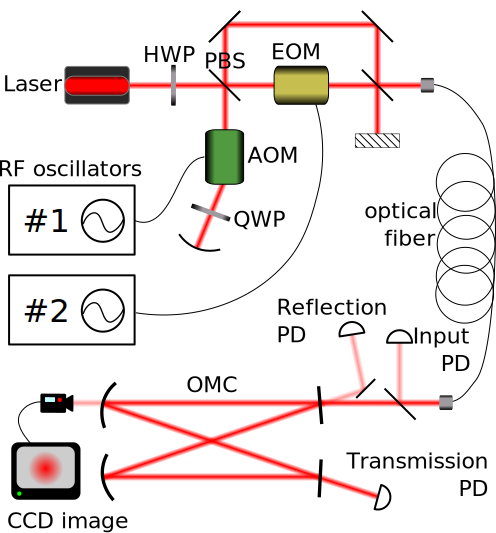
\includegraphics{figs-omc/interrogator.pdf}
  \end{center}
  \caption[Block diagram of OMC characterization setup.]{Block diagram of OMC characterization setup, also known as the OMC interrogator. The setup provides single mode laser light with RF sidebands for reflection locking, as well as a subcarrier with a tunable frequency.}
  \label{fig:interrogator}
\end{figure}

Figure \ref{fig:interrogator} shows a diagram of the experimental setup used to measure several parameters of the OMC that was installed on the H1 LIGO interferometer in Hanford, WA. %NL%
These measurements were done prior to the installation of the OMC into the interferometer. %NL%
The laser source is a Nd:YAG NPRO providing a 1064nm wavelength laser beam. %NL%
The polarization is rotated by a half-wave plate (HWP). %NL%
A polarizing beam splitter (PBS) sends some fraction of the light through an electro-optic modulator (EOM) which is driven at by RF oscillator \#2. %NL%
The fraction transmitted by the PBS is tuned by changing the angle of the HWP. %NL%
The EOM introduces two RF sidebands which will be used for cavity length control. %NL%
The other path of light is directed to an acousto-optic modulator (AOM). %NL%
The light is double passed though the AOM and and receives a frequency shift which is twice the frequency of RF oscillator \#1. %NL%
A quarter-wave plate (QWP) causes the polarization to rotate 90\degrees{} after double passing, causing both paths to now be in the same polarization. %NL%
The light from the two paths are recombined before being injected into an optical fiber. %NL%
The frequency makeup of the combined beam includes the original carrier frequency, two RF sidebands and a frequency shifted subcarrier.

The light exiting the other end of the optical fiber is incident on the input coupling mirror of the OMC cavity. %NL%
A small sample of the input beam is incident on a photodetector. %NL%
The promptly reflected beam is detected on a photodetector where the photocurrent is demodulated at the frequency of RF oscillator \#2 for a PDH style locking scheme. %NL%
The frequency of oscillator \#2 is chosen so that it is outside of the OMC resonance when the carrier is in resonance. %NL%
This provides an error signal which is fed back to the frequency actuator of the laser. %NL%
The control system is able to maintain resonance of the laser in the OMC. %NL%
The laser transmitted through the OMC is detected on another photodetector. %NL%
A very small sample of the light in the cavity is transmitted through one of the HR mirrors and detected by a CCD sensor.

\subsection{Free spectral range}
\label{sec:FSR}
Resonance occurs in the cavity when the total round trip phase of the incident laser beam as it propagates through the cavity is an integer multiple of $2\pi$. %NL%
In terms of the frequency of the laser beam, this occurs at multiples of what is called the \emph{free spectral range} (FSR). %NL%
The FSR is related to the round trip cavity perimeter $p$ by $\mathrm{FSR}=c/p$.

The technique used to measure the cavity FSR involved locking the laser frequency so the carrier was resonant in the OMC while varying the frequency of the subcarrier, causing it to pass through resonance, and measuring the OMC transmitted power. %NL%
The OMC transmitted power will be maximized when the subcarrier is separated from the carrier by a multiple of the FSR.

The RF frequency generator was tuned to maximize the subcarrier transmission. %NL%
The error was estimated to be the smallest frequency step that did not cause a noticeable change in transmission. %NL%
The measured FSR is
\begin{equation}
\mathrm{FSR}=278.288\pm0.001\text{MHz}.
\end{equation}
This corresponds to a cavity perimeter of 1.077m. %NL%
The length differs from the design value, though the purpose of the design was that the fourth order modes are close to, but outside of resonance, as measured in the following section.

\subsection{Higher order mode spacing}
Similarly, the higher order mode frequency shift is measured by varying the subcarrier frequency until the subcarrier is resonant on a higher order mode of the OMC \cite{Uehara:95}. %NL%
Coupling of the subcarrier beam into the HOMs is enhanced if slight misalignments are introduced on the input beam. %NL%
The identity of the higher order mode is determined by the image recorded by the CCD camera.

The HOM field components experience an effective frequency shift relative to the \TEM{00} carrier field due to the Gouy phase shift. %NL%
The effective frequency shift is given by
\begin{equation}
\label{eqn:gouyshift}
(m+n)\eta=\pi\frac{\Delta f}{\mathrm{FSR}}\mod \pi
\end{equation}
where $m$ and $n$ are the \TEM{mn} mode indices, $\Delta f$ is the frequency shift, and $\eta$ is the Gouy phase shift, which is related to the cavity $g$-parameter by Equation \ref{eqn:gouyg}. %NL%


\begin{table}
  \begin{center}
    \begin{tabular}{lll|ll}
      \hline
      $m$ & $n$ & $\Delta f$ & $\eta$ & $g$ \\
      \hline
      0 & 1 & -489.60 MHz & 0.2407$\pi$ & 0.7275\\
      1 & 0 & -489.12 MHz & 0.2424$\pi$ & 0.7238\\
      0 & 4 &  267.96 MHz & 0.2407$\pi$ & 0.7274\\
      4 & 0 &  269.60 MHz & 0.2422$\pi$ & 0.7242\\
      \hline
    \end{tabular}
  \caption[Higher order mode frequency shifts in the OMC]{Higher order mode frequency shifts in the OMC. The frequency shift measured by varying the subcarrier separation from the resonating carrier. The $m$ index is the horizontal mode order. Negative frequency shifts were achieved by using the -1 diffraction order of the AOM.}
  \label{tab:HOM}
  \end{center}
\end{table}

Table \ref{tab:HOM} shows the measurements for several higher order mode frequency shifts. %NL%
Notice that the horizontal and vertical modes experience slightly different Gouy shifts in the cavity. %NL%
This is due to the astigmatism introduced in the cavity by non-normal incidence on the cavity mirrors. %NL%
One may use the measured $g$-parameters to estimate the radius of curvature of the curved optics of the OMC. %NL%
If we take the average value of the measured $g$-parameter, this implies a radius of curvature of 1.96m, which is close to the specification of 2m.

These data were taken with the OMC at room temperature. %NL%
It was later discovered that the HOM spacing varied with the temperature of the thermal length actuator \cite{OTASmodes}\footnote{Note that all ilog references may be viewed publically with username {\it reader} and password {\it readonly}.}. %NL%
With high enough temperature, this would bring the fourth order modes in coincidence resonance with the \TEM{00} mode! %NL%
We postulated that this was due to a change in the effective radius of curvature of the OTAS mirror as the OTAS expanded. %NL%
To mitigate this, the temperature was kept low during operation.

\subsection{Cavity finesse}
\label{sec:finesse}
The frequency profile of the transmitted peak when the subcarrier is shifted through resonance may be used to determine the cavity finesse. %NL%
The finesse is defined as the ratio of the spacing between resonances (the FSR) to the full width at half maximum (FWHM) of the resonance. %NL%
In the experiment, a sawtooth wave was used to sweep the subcarrier offset frequency while the OMC transmission was monitored. %NL%
These signals were digitized and recorded. %NL%
The recorded transmission versus frequency shift data are shown in Figure \ref{fig:finesseFit}. %NL%
The curve fit model used was Equation \ref{eqn:finesse} with $\phi=\pi \Delta f/\mathrm{FSR}$ and an arbitrary scaling and offset. %NL%
The fitting parameters return a cavity finesse of $367\pm2$.


\begin{figure}[h!]
  \begin{center}
  \leavevmode
  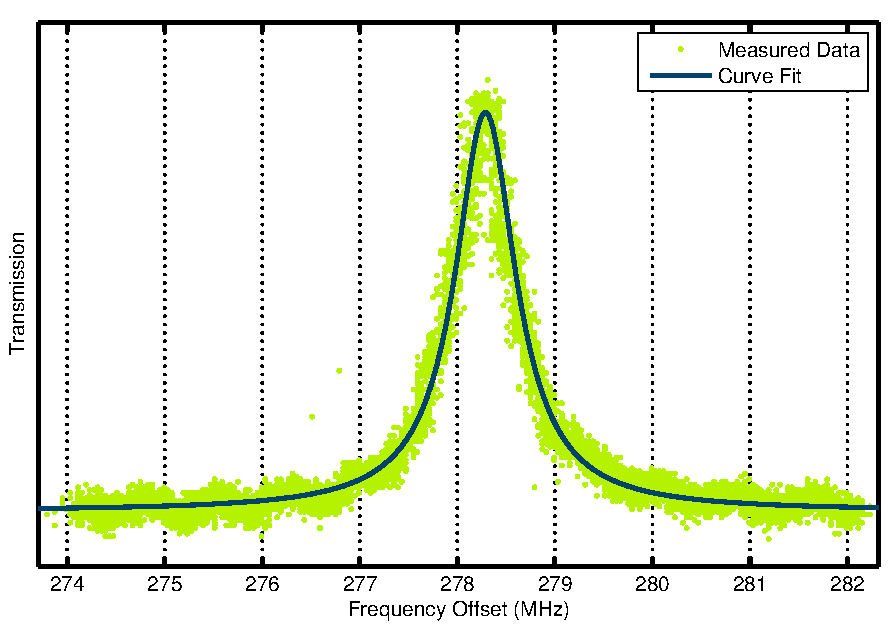
\includegraphics{figs-omc/finesseFit.pdf}
  \end{center}
  \caption[Measurement of the OMC transmission profile.]{Measurement of the OMC transmission profile. The OMC is locked on the carrier, pictured is the transmission while varying frequency offset as the subcarrier passes through resonance. The width of the transmission peak is used to determine the cavity finesse. Fitted parameters give a finesse of $367\pm2$.}
  \label{fig:finesseFit}
\end{figure}

\subsection{Cavity losses}
\label{sec:omclosses}
The intra-cavity loss of the OMC was inferred by using three photodetectors; one measuring a sample of the input light, one measuring the reflected light, and one measuring the transmitted light, as seen in Figure \ref{fig:interrogator}. %NL%
Both the reflection and transmission photodiodes were calibrated relative to the input diode. %NL%
The calibration of the reflection diode was achieved by leaving the input and reflection diodes in place and blocking the beam inside the cavity. %NL%
The relative power readings of the diodes were then recorded and the ratio gives the reflection calibration. %NL%
One must also take into account the known transmission of the OMC input coupling mirror. %NL%
This calibration is done without moving the beam to be used during the measurement and mitigates systematic errors due to variations in the sensitivity over the surface of the diodes. %NL%
The transmission diode, however needed to be moved during calibration to measure the power incident on the cavity. %NL%
The transmission diode was also calibrated relative to the input diode.

This technique measures the light incident on the cavity, reflected from the cavity, and transmitted by the cavity. %NL%
Any incident light which is neither reflected nor transmitted is assumed to be absorbed and constitutes cavity losses. %NL%
Table \ref{tab:lossmeas} shows the data taken to determine the cavity losses. %NL%
The transmission efficiency is defined to be $P_{\text{transmission}}/(P_{\text{input}}-P_{\text{reflection}})$. %NL%
The cavity transmission efficiency was measured to be approximately 96\perc{}.

\begin{table}
  \begin{center}
    \begin{tabular}{lll|l}
      \hline
      Input (V) & Reflection (V) & Transmission (V) & Transmission Efficiency \\
      \hline
      0.95 & 1.51 & 0.53 & 0.965 \\
      0.903 & 1.44 &0.498 & 0.958\\
      \hline
    \end{tabular}
  \caption[Measurements of the OMC intra-cavity losses.]{Measurements of the OMC intra-cavity losses. All units are calibrated in Volts measured by the input PD.}
  \label{tab:lossmeas}
  \end{center}
\end{table}

In September 2010, during the Sixth LIGO Science run, it was discovered that the output efficiency of the H1 interferometer had somehow degraded to below 80\perc{}. %NL%
After the end of the Science Run, this efficiency was determined to originate in the OMC. %NL%
The cause of the degradation was that the position of the OTAS had become mechanically displaced. %NL%
The reason of the displacement is not known but seems to have occurred simultaneously with a site wide power outage at the LIGO Hanford Observatory. %NL%
The beam clearance of the OTAS was very tight and the displacement caused significant beam clipping, leading to losses in the OMC cavity \cite{T1100562}.

\subsection{PZT actuator response}
\begin{figure}[h!]
  \begin{center}
  \leavevmode
  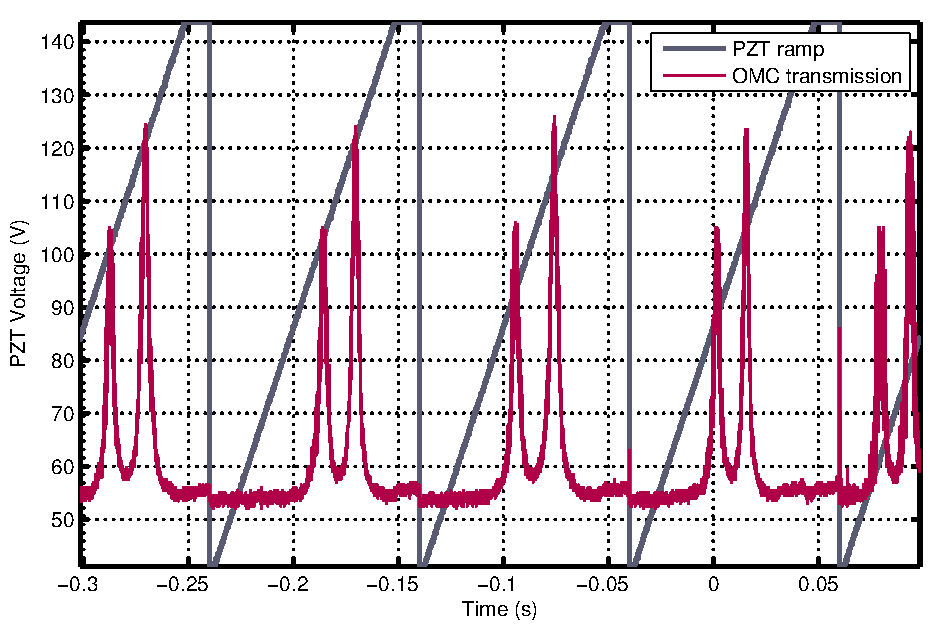
\includegraphics{figs-omc/pztdccal.pdf}
  \end{center}
  \caption[Measurement of the OMC PZT actuator calibration.]{Measurement of the OMC PZT actuator calibration. Both the carrier and subcarrier can be seen passing through resonance.}
  \label{fig:pztsweep}
\end{figure}
The PZT length actuator of the OMC was calibrated by applying a voltage to the PZT to sweep the cavity through both carrier and subcarrier resonances. %NL%
The subcarrier frequency offset was chosen to be close to one FSR separated from the carrier. %NL%
The separation was $1\mathrm{FSR}+3.8$MHz. %NL%
In terms of a change in cavity length, this is 14.5nm, which is twice the distance moved by the mirror. %NL%
Given the known frequency separation of the carrier and subcarrier, a determination of the voltage offset between resonances can be used to calibrate the PZT. %NL%
The data taken are show in Figure \ref{fig:pztsweep}, and the mean offset of the central three ramps is 19.8V. %NL%
Thus the PZT calibration is $\frac{14.5\text{nm}}{2}\frac{1}{19.8\text{V}}=0.37\text{nm}/\text{V}$.


\section{Optical feedback instability in the OMC}
\begin{figure}
  \begin{center}
  \leavevmode
  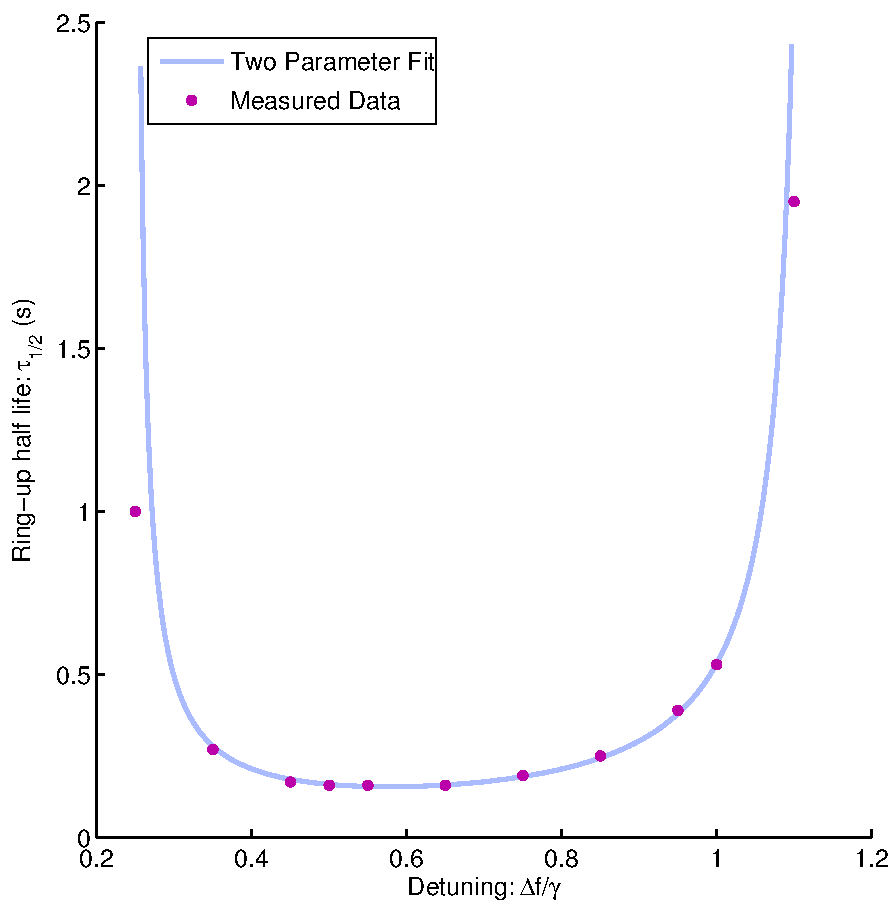
\includegraphics{figs-omc/raddamping.pdf}
  \end{center}
  \caption[Measurement of ring-up times of optical instability in the OMC.]{Measurement of ring-up times of optical instability in the OMC. The instability ring up time was measured for several values of the cavity detuning. Also plotted is a two-parameter curve fit to the data. Data collected by Tim Bodiya and Nicolas Smith-Lefebvre.}
  \label{fig:raddamping}
\end{figure}
An issue arose during Enhanced LIGO which hindered the development of an automatic cavity locking system for the OMC. %NL%
As the OMC was brought into resonance, some kind of dynamical instability would be activated and this would cause signals in the transmitted power at kHz frequencies with amplitudes large enough to saturate the readout electronics. %NL%
Because the locking servo was based on a transmission dither scheme, these instabilities would pollute the cavity length error signal and prevent locking. %NL%
The instabilities would not be excited at the very peak of resonance, so for some fraction of the attempts, there would be a successful lock of the cavity. %NL%
The result of this is that locking the OMC was the only step in the lock acquisition and low noise operation of Enhanced LIGO that was not fully automated during science data taking. %NL%
The lack of an automatic OMC locking system probably had a detrimental effect on the overall duty cycle of the interferometers, but the magnitude of this effect would be difficult to determine.

The mechanism of the instability was never understood. %NL%
It had the following characteristics:
\begin{itemize}
\item The strength of the instability depended on the circulating cavity power. for small power incident on the OMC (less than 1mW) there was no instability.
\item The instability was not coupling through the PZT actuator. The instability remained even with the PZT leads were shorted.
\item There was no instability when the cavity was centered on resonance.
\item There was instability on either side of cavity resonance.
\end{itemize}

There was an attempt to quantify the behavior of this instability by investigating the dependence of the ring-up time of one of the unstable modes with a frequency of 1.1kHz. %NL%
The OMC was locked detuned from resonance with approximately 9mW of power transmitted through the cavity. %NL%
The data that were taken are shown in Figure \ref{fig:raddamping} as the ring-up half life, $\tau_{1/2}$, as a function of cavity detuning, $\Delta f/\gamma$, where $\gamma= \frac{1}{2}\frac{\rm{FSR}}{\mathcal{F}}$ is the cavity linewidth.

Also shown in Figure \ref{fig:raddamping} is a simple model of the ring-up time. %NL%
The model comprises a exponential ring-up characterized by an anti-damping term which has the following functional dependence on the detuning:
\begin{equation}
\label{eqn:gamma}
\Gamma(\Delta f)=\frac{2\Delta f/\gamma}{\left[1+\left(\Delta f/\gamma\right)^2\right]^2},
\end{equation}
which is just the derivative of the cavity transmission profile (Equation \ref{eqn:finesse}) for small $\Delta f$. %NL%
Explicitly, the ring-up half life is
\begin{equation}
\tau_{1/2}=\tau_0\left(\frac{2\Delta f/\gamma}{\left[1+\left(\Delta f/\gamma\right)^2\right]^2}-\Gamma_0\right)^{-1}.
\end{equation}
The best fit of the model to the data is given by $\tau_0=33\pm 6$ms and $\Gamma_0=0.438\pm 0.001$.

Perhaps the most interesting aspect about the model is what mechanism it rules out. %NL%
An opto-mechanical parametric instability driven by radiation pressure would have a third factor of $\left[1+\left(\Delta f/\gamma\right)^2\right]$ in the denominator for Equation \ref{eqn:gamma} \cite{Corbitt:7mK}. %NL%
A curve fit with a model consistent with a radiation pressure instability was also tried, but did not provide a good agreement with the data. %NL%
So although it seems that the instability is somehow driven by the intra-cavity power, it is not consistent with radiation pressure.

Ultimately this did not pose a problem for the noise performance of the interferometer, because the OMC is always kept on resonance during normal operation, it is not operated detuned. %NL%
However, it did remain a poorly understood feature of the system and because Advanced LIGO will use the same, or a similar OMC, it likely warrants further investigation.

\section{OMC performance in Enhanced LIGO and prospects for future interferometers}

The ultimate performance of the interferometer is affected by the OMC in several ways. %NL%
The ability of the OMC to maximally transmit the gravitational wave signal directly affects the shot-noise limited SNR of the interferometer (this is covered in Section \ref{sec:alignsnr}). %NL%
Losses inside the OMC will limit the transmission, but these were shown to be low (Section \ref{sec:omclosses}). %NL%
A more subtle problem is to correctly match the incident beam to the resonant \TEM{00} mode of the OMC, any signal light which is not correctly matched will be rejected. %NL%
From the point of the readout sensitivity, this is effectively a loss. %NL%
The two most common forms of cavity mismatch are alignment (Chapter \ref{ch:beacon}) and mode matching (Chapter \ref{ch:modematching}). %NL%
In addition to signal losses, the addition of an OMC can bring new noise couplings, perhaps the most important being the sensitivity to beam jitter (Chapter \ref{ch:jitter}).

\begin{figure}[h!]
  \begin{center}
  \leavevmode
  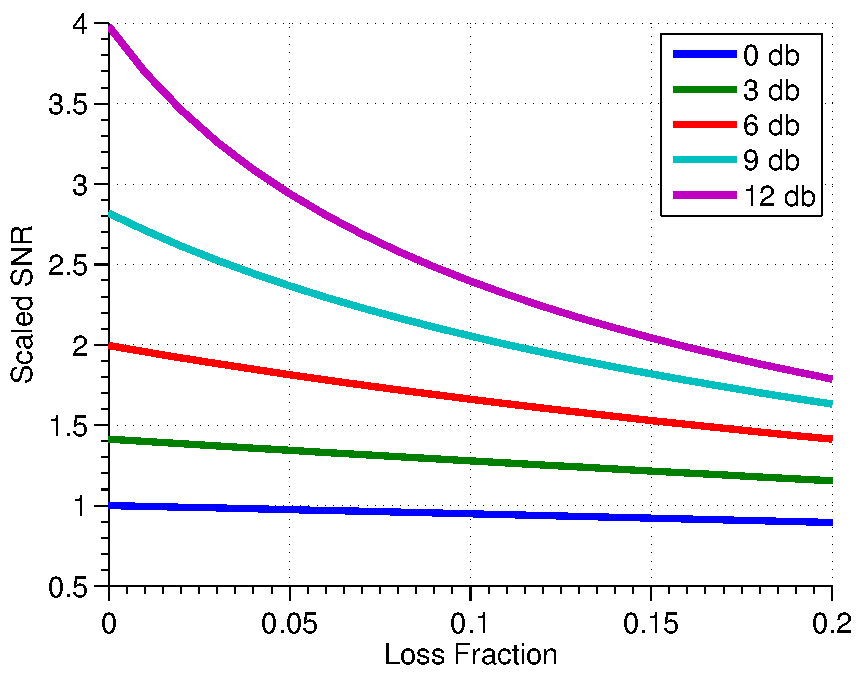
\includegraphics{figs-omc/squeezeplot.pdf}
  \end{center}
  \caption[Interferometer readout SNR gain from squeezing as a function of output losses.]{Interferometer readout SNR gain from squeezing as a function of output losses. Higher levels of squeezing lead to increased sensitivity to output losses, including those from the OMC.}
  \label{fig:squeezeplot}
\end{figure}

An analysis of the readout sensitivity of the two Enhanced LIGO interferometers was performed by \citet{Tobin}. %NL%
This analysis showed that both interferometers performed at the expected level of sensitivity when all known output losses were taken into account. %NL%
The OMCs thus provided the desired outcome of improving the ultimate interferometer sensitivity. %NL%
One of the major sources of loss for the H1 interferometer was mode mismatching, this was the motivation for the system proposed in Chapter \ref{ch:modematching}.

The use of squeezed light to further enhance the readout sensitivity of laser interferometers has recently been demonstrated as both feasible and practical on full scale gravitational wave antennae \cite{GEOSqz:11,LIGOSqz}. %NL%
Output losses become even more important when the interferometer employs squeezed light injection. %NL%
Figure \ref{fig:squeezeplot} shows how losses in the readout chain can degrade the interferometer sensitivity for different levels of squeezed light injection. %NL%
The prospects of squeezing for future interferometers certainly offer great promise for boosting interferometer sensitivity. %NL%
Although, these benefits can only be fully exploited if the output losses are maintained at a minimal level. %NL%
The performance of the OMC is central to realizing these goals.

The following chapter covers some theoretical background necessary for analyzing how the OMC interacts with the output beam of the interferometer.
